%%
%% Copyright 2007, 2008, 2009 Elsevier Ltd
%%
%% This file is part of the 'Elsarticle Bundle'.
%% ---------------------------------------------
%%
%% It may be distributed under the conditions of the LaTeX Project Public
%% License, either version 1.2 of this license or (at your option) any
%% later version.  The latest version of this license is in
%%    http://www.latex-project.org/lppl.txt
%% and version 1.2 or later is part of all distributions of LaTeX
%% version 1999/12/01 or later.
%%
%% The list of all files belonging to the 'Elsarticle Bundle' is
%% given in the file `manifest.txt'.
%%

%% Template article for Elsevier's document class `elsarticle'
%% with numbered style bibliographic references
%% SP 2008/03/01
%%
%%
%%
%% $Id: elsarticle-template-num.tex 4 2009-10-24 08:22:58Z rishi $
%%
%%
%%\documentclass[preprint,12pt,3p]{elsarticle}

%% Use the option review to obtain double line spacing
%%\documentclass[preprint,review,12pt]{elsarticle}

%% Use the options 1p,twocolumn; 3p; 3p,twocolumn; 5p; or 5p,twocolumn
%% for a journal layout:
%% \documentclass[final,1p,times]{elsarticle}
%% \documentclass[final,1p,times,twocolumn]{elsarticle}
%% \documentclass[final,3p,times]{elsarticle}
\documentclass[final,3p,times,twocolumn]{elsarticle}
%% \documentclass[final,5p,times]{elsarticle}
%% \documentclass[final,5p,times,twocolumn]{elsarticle}

%% if you use PostScript figures in your article
%% use the graphics package for simple commands
%% \usepackage{graphics}
%% or use the graphicx package for more complicated commands
%% \usepackage{graphicx}
%% or use the epsfig package if you prefer to use the old commands
%% \usepackage{epsfig}


%% The amssymb package provides various useful mathematical symbols
\usepackage{blindtext, graphicx, amsmath, algorithm, algpseudocode, pifont, algcompatible, comment, layout, amsthm, amssymb}
\usepackage{enumitem}   
\usepackage{eso-pic}
\usepackage{booktabs}
\usepackage{float}
%% The amsthm package provides extended theorem environments
%% \usepackage{amsthm}
\renewcommand{\qedsymbol}{$\blacksquare$}

\usepackage[utf8]{inputenc}
\usepackage[english]{babel}
\usepackage{hyperref} 
\hypersetup{ colorlinks=true, linkcolor=black, filecolor=black, urlcolor=cyan, }

\usepackage{caption}
\captionsetup{justification=raggedright, singlelinecheck = false}
\captionsetup[table]{labelformat=simple, labelsep=newline}
\captionsetup[figure]{labelformat=simple, labelsep=period}


%% The lineno packages adds line numbers. Start line numbering with
%% \begin{linenumbers}, end it with \end{linenumbers}. Or switch it on
%% for the whole article with \linenumbers after \end{frontmatter}.
%% \usepackage{lineno}

%% natbib.sty is loaded by default. However, natbib options can be
%% provided with \biboptions{...} command. Following options are
%% valid:

%%   round  -  round parentheses are used (default)
%%   square -  square brackets are used   [option]
%%   curly  -  curly braces are used      {option}
%%   angle  -  angle brackets are used    <option>
%%   semicolon  -  multiple citations separated by semi-colon
%%   colon  - same as semicolon, an earlier confusion
%%   comma  -  separated by comma
%%   numbers-  selects numerical citations
%%   super  -  numerical citations as superscripts
%%   sort   -  sorts multiple citations according to order in ref. list
%%   sort&compress   -  like sort, but also compresses numerical citations
%%   compress - compresses without sorting
%%
%% \biboptions{comma,round}

% \biboptions{}
\newtheorem{theorem}{Theorem}
\newtheorem{lemma}{Lemma}
\newtheorem{definition}{Definition}

\journal{ICT Express}

%\newcommand\AtPagemyUpperRight[1]{\AtPageLowerRight{%
%\put(\LenToUnit{0.8\paperwidth},\LenToUnit{0.9\paperheight}){#1}}}
%\AddToShipoutPictureFG{
%  \AtPagemyUpperRight{{\includegraphics[width=.5cm,keepaspectratio]{logo.png}}}
%}%
%\newcommand\AtPagemyUpperLeft[1]{\AtPageLowerLeft{%
%\put(\LenToUnit{0.85\paperwidth},\LenToUnit{0.9\paperheight}){#1}}}
%\AddToShipoutPictureFG{
%  \AtPagemyUpperLeft{{\includegraphics[width=1.0cm,keepaspectratio]{logo2.jpg}}}
%}%
\begin{document}

\begin{frontmatter}

\title{Submission Guideline for ICT Express}
%\author{Author’s Full Name 1\corref{cor1}, Author’s Full Name 2, Author’s Full Name 3}
\author{Author’s Full Name 1\corref{cor1}}
\ead{author1@ictexpress.com}

\author{Author’s Full Name 2}
\ead{author2@ictexpress.com}

\author{Author’s Full Name 3}
\ead{author3@ictexpress.com}
\address{Department, Organization, City, Country\\Department, Organization, City, Country\\Department, Organization, City, Country}

\cortext[cor1]{Corresponding author}
%\ead{author1@ictexpress.com, author2@ictexpress.com, author2@ictexpress.com}



\begin{abstract}
The abstract should be self-contained (contains no footnotes). It should concisely state what was done, how it was done, principal results, and their significance. It should be around 75 to 100 words for all forms of publication. The abstract should be written as one paragraph and should not contain displayed mathematical equations, tabular materials, or numbered references. At the end of abstract, index terms should be given in 3 to 5 keywords and in alphabetical order, separated by semi-colons. 
\\
2018 The Korean Institute of Communications and Information Sciences. Publishing Services by Elsevier B.V. This is an open access article under the CC BY-NC-ND license (http://creativecommons.org/licenses/by-nc-nd/4.0/).
\end{abstract}

\begin{keyword}
%% keywords here, in the form: keyword \sep keyword
ICT Express \sep Submission guideline \sep Template 
%% MSC codes here, in the form: \MSC code \sep code
%% or \MSC[2008] code \sep code (2000 is the default)
\end{keyword}

\end{frontmatter}

%%
%% Start line numbering here if you want
%%
% \linenumbers

%% main text
\section{Introduction}\label{sec1}
ICT Express publishes original research papers in English in the fields of ICT convergence, platform technologies, communication networks, and device technologies. 
ICT Express accepts short-length high-quality, original articles in Latex or Word format. 
Manuscript must be submitted by one of its authors on behalf of all the authors. The submitting author takes responsibility for the article during submission and peer review. 

The authors are required to upload the manuscript as a PDF file at the time of submission. 
Using MS Word or LaTeX template, the length of the letter is recommended as 4 pages including title, list of authors, abstract, figures, tables, and references. 
Figures and tables are allowed up to 4 in total. Each manuscript must be accompanied by an abstract in 75 to 100 words and a list of 3 to 5 keywords. 
Submitted manuscripts violating these guidelines will be returned to the authors without being reviewed. 
\vspace{1.3cm}

The author(s) or his/her/their company or institution will be billed $\$$100 per each page in excess of the first four published pages. 
The author(s) signifies his willingness to pay these charges simply by submitting his/her/their manuscript to the ICT Express. 
The Publisher holds the right to withhold publication under any circumstance, as well as publication of the current or future submissions of authors who have outstanding mandatory page charge debt. 
No mandatory overlength page charges will be applied to overview articles or invited articles. 

\section{Manuscript Preparation}\label{sec2}
\subsection{Format of initial or intermediate contributions}
The main document with the manuscript text, figures, and tables should be prepared in an MS World or LaTeX format in English. 
The manuscript should be written in 10-point font with single line spacing on A4 sized (21.0 x 29.7 cm) paper with 1.3 cm margins on the top, bottom, right, and left. 
The standard order of sections in the manuscript is title page, abstract, introduction, system model and methods, results, discussion, references. 
Figures and tables with legends should be embedded in the proper place in the text. 
The number of all manuscript pages should be specified, starting with the title page as page 1. A single file is permitted for initial submission, but figures and tables can be uploaded separately.

\begin{table}[]
%\footnotesize
\centering
\caption{An example of a table.}
\begin{tabular}{@{}lcc@{}}
\toprule
Column heading & Column A & Column B \\ \midrule
And an entry                   & 1        & 2        \\
And another entry              & 3        & 4        \\
And another entry              & 5        & 6        \\
And another entry              & 7        & 8        \\ \bottomrule
\end{tabular}
\label{tab:ex}
\end{table}

\subsection{Title page}

The Title page should include a full title, running title (no more than 40 characters in length) of the article and authors' information. \\

\textbf{Title. }should be as concise as possible but informative enough to facilitate information retrieval.\\

\textbf{Author names and affiliations. }Please clearly indicate the given name(s) and family name(s) of each author and check that all names are accurately spelled. 
Present the authors' affiliation addresses (where the actual work was done) below the names. 
Indicate all affiliations with a lower-case superscript letter immediately after the author's name and in front of the appropriate address. 
Provide the full postal address of each affiliation, including the country name and, if available, the e-mail address of each author.\\

\textbf{Corresponding author. }Clearly indicate who will handle correspondence at all stages of refereeing and publication, also post-publication. 
This responsibility includes answering any future queries. 
Ensure that the e-mail address is given and that contact details are kept up to date by the corresponding author.\\

\textbf{Present/permanent address. }If an author has moved since the work described in the article was done, or was visiting at the time, a 'Present address' (or 'Permanent address') may be indicated as a footnote to that author's name. 
The address at which the author actually did the work must be retained as the main affiliation address. 
Superscript Arabic numerals are used for such footnotes.

\subsection{Text}

The text is recommended to be arranged in this order, if possible: Introduction, System Model and Methods, Result, Discussion, and Conclusions.\\

\textbf{Introduction.} the purpose and the background should be written simply and lucidly. \\

\textbf{System Model and Methods.} the methodology should be written precisely so that others may use some or all of the methods in another study or judge the scientific merit of your work.\\

\begin{figure}
\centering
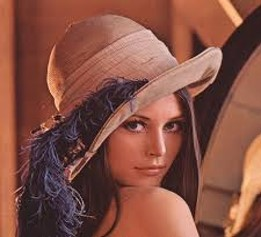
\includegraphics[width=.8\columnwidth]{fig1.jpg}
\caption{Example of a figure.}
\label{fig:ex}
\end{figure}

\textbf{Result.} a detailed description of the study results should be objectively presented, in an orderly and logical sequence using both text and illustrative materials (Tables and Figures). \\

\textbf{Discussion and Conclusions.} author's interpretation of the results, author's opinion. Conclusion should be written simply.

\subsection{Text section heading}
Divide your article into clearly defined and numbered sections. 
Subsections should be numbered as 1.1 (then 1.1.1, 1.1.2, ...), 1.2, etc. (the abstract is not included in the section numbering). 
Use this numbering also for internal cross-referencing. Any subsection may be given a brief heading. 
Each heading should appear on its own separate line.

\subsection{References in text}
References should be obviously related to documents. 
Indicate references by number(s) in square brackets in line with the text. 
The numbered references are listed in the order in which they appear in the text.
The actual authors can be referred to, but the reference number(s) must always be given. Example: '..... as demonstrated [3,6]. 
Barnaby and Jones [8] obtained a different result ....'

\subsection{Text equations}

The Equations should be punctuated and aligned to bring out their structure and numbered on the right as
\begin{equation}
y = Hx+n.
\end{equation}

Mathematical operation signs indicating continuity of the expression should be placed at the left of the second and succeeding lines. 
Use $\times$ rather than a centered dot, except for scalar products of vectors. 
The solidus ($\slash$) should be used instead of built-up fractions in running text. 
Furthermore, the Notation must be legible, clear, compact, and consistent with standard usage. 
All unusual symbols whose identity may not be obvious must be identified when they first appear, and whenever confusion might arise. 
Superscripts are normally set directly over subscripts; authors should note where readability or the meaning requires a special order. 
In the text, numbers should be Arabic numerals, except when beginning a sentence. 
Numbers greater than 999 should have commas, e.g., 13,970. 
The 24-hour system is used to indicate time, e.g., 18:00 hr. 
If you are using Word for Math, use either the Microsoft Equation Editor or the MathType add-on (\url{http://www.mathtype.com}) for equations in your paper.
“Float over text” should not be selected.

\subsection{Units and abbreviations}
Units of measure should be presented according to the International System (SI) of Units. If other units are mentioned, please give their equivalent in SI.

Abbreviations must be used as an aid to the reader, rather than as a convenience of the author, and therefore their use should be limited. 
Acronyms and abbreviations should be defined at the first time when they are used in text.

\subsection{Tables}
Each Table should be numbered with Arabic numerals in the order of their appearance in the text. 
Tables should have a concise and informative title with the table content between horizontal lines. 
The structure should be clear, with simple column headings giving all units. 
A table should not exceed one page when printed. Use lower case letters in superscripts a, b, c ... for special remarks. 
An example of a table is given in Table \ref{tab:ex}.

\subsection{Figures}
Figures are numbered consecutively in the sequence mentioned in the text and must have a caption written in one paragraph style. 
The caption should contain an explanation of all abbreviations and symbols used, and indicate the size value of lines or bars unless shown directly on the figure. 
An example of a figure is given in Fig. \ref{fig:ex}. 
The Figure number should be placed at the lower-left corner of each figure, and the numbering order must be from left to right, and from upper to lower. 
Citations of figures in the text or parentheses are abbreviated, e.g., Fig. 1, Figs. 1 and 2, Figs. 1-3, (Fig. 1), (Figs. 1 and 2), (Figs. 1-3). 
When the text refers to both figures and tables, they should be mentioned in parentheses, e.g., (Table 1; Fig. 2) and (Tables 1-3; Figs. 4-6).

\subsection{Footnotes}
Footnotes should be used sparingly. Number them consecutively throughout the article. 
Many word processors can build footnotes into the text, and this feature may be used. 
Otherwise, please indicate the position of footnotes in the text and list the footnotes themselves separately at the end of the article. 
Do not include footnotes in the Reference list.


\section*{Acknowledgments}
Collate acknowledgements in a separate section at the end of the article before the references and do not, therefore, include them on the title page, as a footnote to the title or otherwise.
List here those individuals who contributed to the papers but not enough to be coauthors may be introduced. 
Financial support, including foundations, institutions, pharmaceutical and device manufacturers, private companies, intramural departmental sources, or any other support should be described.

\section*{Appendix}
Appendix section should be placed before References section. 
If there is more than one appendix, they should be identified as A, B, etc. 
Formulae and equations in appendices should be given with separate numbering: Eq. (A.1), Eq. (A.2), etc.; in a subsequent appendix, Eq. (B.1) and so on. 
The numbering of tables and figures in the appendix is similar: Table A.1; Fig. A.1, etc.

\section*{Conflict of interest}
The authors declare that there is no conflict of interest in this paper.

%% References
%%
%% Following citation commands can be used in the body text:
%% Usage of \cite is as follows:
%%   \cite{key}         ==>>  [#]
%%   \cite[chap. 2]{key} ==>> [#, chap. 2]
%%

%% References with bibTeX database:

\bibliographystyle{elsarticle-num}
% \bibliographystyle{elsarticle-harv}
% \bibliographystyle{elsarticle-num-names}
% \bibliographystyle{model1a-num-names}
% \bibliographystyle{model1b-num-names}
% \bibliographystyle{model1c-num-names}
% \bibliographystyle{model1-num-names}
% \bibliographystyle{model2-names}
% \bibliographystyle{model3a-num-names}
% \bibliographystyle{model3-num-names}
% \bibliographystyle{model4-names}
% \bibliographystyle{model5-names}
% \bibliographystyle{model6-num-names}

\vspace{-0.3cm}

\begin{thebibliography}{1}

\bibitem{els} H. Kwon, K. Kim, C. Lee, The unified UE baseband modem hardware platform architecture for 3GPP specification, J. Commun. Net., 13 (1) (2011) 70-76.

\bibitem{els} T. Roos, P. Myllymaki, H. Tirri, A statistical modeling approach to location estimation, IEEE Trans. Mobile Comput. 1 (1) (2002) 59-69.

\bibitem{els} H. Liu, G. Li, OFDM-Based Broadband Wireless Networks: Design and Optimization. Hoboken, NJ: Wiley-Interscience, 2005.

\bibitem{els} T. L. Marzetta, How much training is required for multiuser MIMO?, in: 2006 Asilomar Conf. Signal. Syst. Comput., Pacific Grove, 2006, pp. 359–363.

\bibitem{els} J. Arrillaga, B. Giessner, Limitation of short-circuit levels by means of HVDC links, in: 1990 IEEE Summer Power Meeting, Los Angeles, 1990, pp. 1-8.

\bibitem{els} J. O. Williams, Narrow-band analyzer, Ph.D. dissertation, Dept. Elect. Eng., Harvard Univ., Cambridge, MA, 1993.

\bibitem{els} J. H. Davis, J. R. Cogdell, Calibration program for the 16-foot antenna, Elect. Eng. Res. Lab., Univ. Texas, Austin, Tech. Memo. NGL-006-69-3, Nov. 15, 1987.

\bibitem{els} RealVNC Ltd. Remote control software [Online]. Available: http:// www.realvnc.com


\end{thebibliography}
\end{document}

%%
%% End of file `elsarticle-template-num.tex'.
